\documentclass[border=2mm]{standalone}
\usepackage{tikz}
\usepackage{tabu}

\begin{document}

\begin{tabu} to \textwidth{|c|c|}
\hline
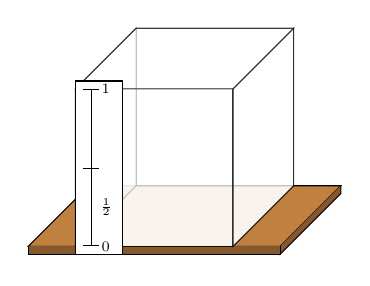
\begin{tikzpicture}[scale=2]

\draw [fill=brown] (-.3,0,0) -- (1.3,0,0) -- (1.3,0,1) -- (-.3,0,1) -- cycle;
\draw [fill=brown!70!black] (1.3,0,-0) -- (1.3,-.05,0) -- (1.3,-.05,1) -- (1.3,0,1);
\draw [fill=brown!70!black] (1.3,0,1) -- (1.3,-.05,1) -- (-.3,-.05,1) -- (-.3,0,1);

\draw [fill=white, opacity=.7] (0,0,0) -- (1,0,0) -- (1,0,1) -- (0,0,1) -- cycle;
\draw [fill=white, opacity=.7] (0,0,0) -- (0,1,0) -- (1,1,0) -- (1,0,0) -- cycle;
\draw [fill=white, opacity=.7] (0,0,0) -- (0,1,0) -- (0,1,1) -- (0,0,1) -- cycle;
\draw [fill=white, opacity=.7] (0,0,1) -- (1,0,1) -- (1,1,1) -- (0,1,1) -- cycle;
\draw [fill=white, opacity=.7] (1,0,0) -- (1,0,1) -- (1,1,1) -- (1,1,0) -- cycle;
\draw [fill=white, opacity=.7] (0,1,0) -- (1,1,0) -- (1,1,1) -- (0,1,1) -- cycle;

\filldraw [fill=white] (0,-.05,1) rectangle (0.3,1.05,1);
\draw [|-|] (.1,0,1) -- (.1,1,1) node [right, scale=.75, xshift=.05cm] {\scriptsize 1} node [ right, pos=0, scale=.75, xshift=.05cm]{\scriptsize 0};
\draw [|-|] (.1,0,1) -- (.1,.5,1) node [right, scale=.75, xshift=.025cm,pos=.5] {\scriptsize $\frac{1}{2}$};

\end{tikzpicture}

& 

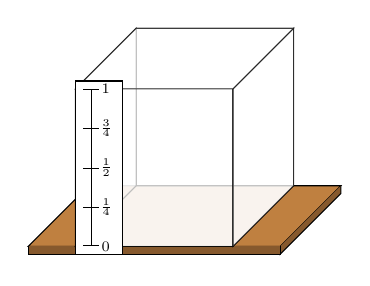
\begin{tikzpicture}[scale=2]

\draw [fill=brown] (-.3,0,0) -- (1.3,0,0) -- (1.3,0,1) -- (-.3,0,1) -- cycle;
\draw [fill=brown!70!black] (1.3,0,-0) -- (1.3,-.05,0) -- (1.3,-.05,1) -- (1.3,0,1);
\draw [fill=brown!70!black] (1.3,0,1) -- (1.3,-.05,1) -- (-.3,-.05,1) -- (-.3,0,1);



\draw [fill=white, opacity=.7] (0,0,0) -- (1,0,0) -- (1,0,1) -- (0,0,1) -- cycle;
\draw [fill=white, opacity=.7] (0,0,0) -- (0,1,0) -- (1,1,0) -- (1,0,0) -- cycle;
\draw [fill=white, opacity=.7] (0,0,0) -- (0,1,0) -- (0,1,1) -- (0,0,1) -- cycle;
\draw [fill=white, opacity=.7] (0,0,1) -- (1,0,1) -- (1,1,1) -- (0,1,1) -- cycle;
\draw [fill=white, opacity=.7] (1,0,0) -- (1,0,1) -- (1,1,1) -- (1,1,0) -- cycle;
\draw [fill=white, opacity=.7] (0,1,0) -- (1,1,0) -- (1,1,1) -- (0,1,1) -- cycle;

\filldraw [fill=white] (0,-.05,1) rectangle (0.3,1.05,1);
\draw [|-|] (.1,0,1) -- (.1,1,1) node [right, scale=.75, xshift=.05cm] {\scriptsize 1} node [ right, pos=0, scale=.75, xshift=.05cm]{\scriptsize 0};
\draw [|-|] (.1,0,1) -- (.1,.5,1) node [right, scale=.75, xshift=.025cm] {\scriptsize $\frac{1}{2}$};
\draw [|-|] (.1,0,1) -- (.1,.25,1) node [right, scale=.75, xshift=.025cm] {\scriptsize $\frac{1}{4}$};
\draw [|-|] (.1,0,1) -- (.1,.75,1) node [right, scale=.75, xshift=.025cm] { \scriptsize $\frac{3}{4}$};


\end{tikzpicture} \\

\hline


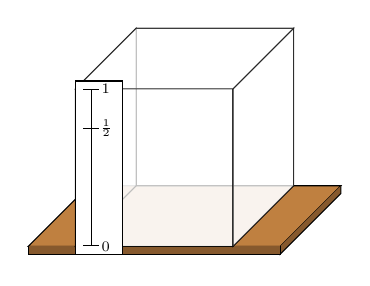
\begin{tikzpicture}[scale=2]

\draw [fill=brown] (-.3,0,0) -- (1.3,0,0) -- (1.3,0,1) -- (-.3,0,1) -- cycle;
\draw [fill=brown!70!black] (1.3,0,-0) -- (1.3,-.05,0) -- (1.3,-.05,1) -- (1.3,0,1);
\draw [fill=brown!70!black] (1.3,0,1) -- (1.3,-.05,1) -- (-.3,-.05,1) -- (-.3,0,1);



\draw [fill=white, opacity=.7] (0,0,0) -- (1,0,0) -- (1,0,1) -- (0,0,1) -- cycle;
\draw [fill=white, opacity=.7] (0,0,0) -- (0,1,0) -- (1,1,0) -- (1,0,0) -- cycle;
\draw [fill=white, opacity=.7] (0,0,0) -- (0,1,0) -- (0,1,1) -- (0,0,1) -- cycle;
\draw [fill=white, opacity=.7] (0,0,1) -- (1,0,1) -- (1,1,1) -- (0,1,1) -- cycle;
\draw [fill=white, opacity=.7] (1,0,0) -- (1,0,1) -- (1,1,1) -- (1,1,0) -- cycle;
\draw [fill=white, opacity=.7] (0,1,0) -- (1,1,0) -- (1,1,1) -- (0,1,1) -- cycle;

\filldraw [fill=white] (0,-.05,1) rectangle (0.3,1.05,1);
\draw [|-|] (.1,0,1) -- (.1,1,1) node [right, scale=.75, xshift=.05cm] {\scriptsize 1} node [ right, pos=0, scale=.75, xshift=.05cm]{\scriptsize 0};

\draw [|-|] (.1,0,1) -- (.1,.75,1) node [right, scale=.75, xshift=.025cm] { \scriptsize $\frac{1}{2}$};


\end{tikzpicture}

& 
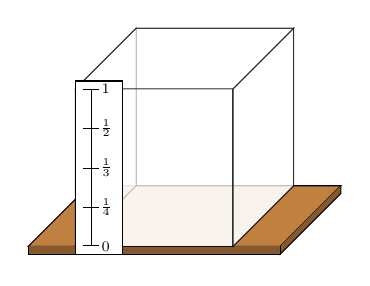
\begin{tikzpicture}[scale=2]

\draw [fill=brown] (-.3,0,0) -- (1.3,0,0) -- (1.3,0,1) -- (-.3,0,1) -- cycle;
\draw [fill=brown!70!black] (1.3,0,-0) -- (1.3,-.05,0) -- (1.3,-.05,1) -- (1.3,0,1);
\draw [fill=brown!70!black] (1.3,0,1) -- (1.3,-.05,1) -- (-.3,-.05,1) -- (-.3,0,1);



\draw [fill=white, opacity=.7] (0,0,0) -- (1,0,0) -- (1,0,1) -- (0,0,1) -- cycle;
\draw [fill=white, opacity=.7] (0,0,0) -- (0,1,0) -- (1,1,0) -- (1,0,0) -- cycle;
\draw [fill=white, opacity=.7] (0,0,0) -- (0,1,0) -- (0,1,1) -- (0,0,1) -- cycle;
\draw [fill=white, opacity=.7] (0,0,1) -- (1,0,1) -- (1,1,1) -- (0,1,1) -- cycle;
\draw [fill=white, opacity=.7] (1,0,0) -- (1,0,1) -- (1,1,1) -- (1,1,0) -- cycle;
\draw [fill=white, opacity=.7] (0,1,0) -- (1,1,0) -- (1,1,1) -- (0,1,1) -- cycle;

\filldraw [fill=white] (0,-.05,1) rectangle (0.3,1.05,1);
\draw [|-|] (.1,0,1) -- (.1,1,1) node [right, scale=.75, xshift=.05cm] {\scriptsize 1} node [ right, pos=0, scale=.75, xshift=.05cm]{\scriptsize 0};
\draw [|-|] (.1,0,1) -- (.1,.5,1) node [right, scale=.75, xshift=.025cm] {\scriptsize $\frac{1}{3}$};
\draw [|-|] (.1,0,1) -- (.1,.25,1) node [right, scale=.75, xshift=.025cm] {\scriptsize $\frac{1}{4}$};
\draw [|-|] (.1,0,1) -- (.1,.75,1) node [right, scale=.75, xshift=.025cm] { \scriptsize $\frac{1}{2}$};


\end{tikzpicture} \\
\hline

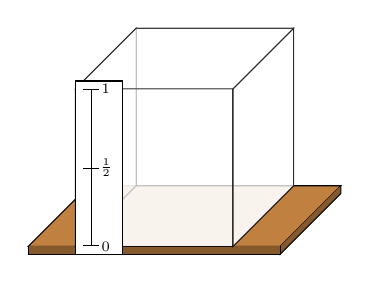
\begin{tikzpicture}[scale=2]

\draw [fill=brown] (-.3,0,0) -- (1.3,0,0) -- (1.3,0,1) -- (-.3,0,1) -- cycle;
\draw [fill=brown!70!black] (1.3,0,-0) -- (1.3,-.05,0) -- (1.3,-.05,1) -- (1.3,0,1);
\draw [fill=brown!70!black] (1.3,0,1) -- (1.3,-.05,1) -- (-.3,-.05,1) -- (-.3,0,1);


\draw [fill=white, opacity=.7] (0,0,0) -- (1,0,0) -- (1,0,1) -- (0,0,1) -- cycle;
\draw [fill=white, opacity=.7] (0,0,0) -- (0,1,0) -- (1,1,0) -- (1,0,0) -- cycle;
\draw [fill=white, opacity=.7] (0,0,0) -- (0,1,0) -- (0,1,1) -- (0,0,1) -- cycle;
\draw [fill=white, opacity=.7] (0,0,1) -- (1,0,1) -- (1,1,1) -- (0,1,1) -- cycle;
\draw [fill=white, opacity=.7] (1,0,0) -- (1,0,1) -- (1,1,1) -- (1,1,0) -- cycle;
\draw [fill=white, opacity=.7] (0,1,0) -- (1,1,0) -- (1,1,1) -- (0,1,1) -- cycle;

\filldraw [fill=white] (0,-.05,1) rectangle (0.3,1.05,1);
\draw [|-|] (.1,0,1) -- (.1,1,1) node [right, scale=.75, xshift=.05cm] {\scriptsize 1} node [ right, pos=0, scale=.75, xshift=.05cm]{\scriptsize 0};
\draw [|-|] (.1,0,1) -- (.1,.5,1) node [right, scale=.75, xshift=.025cm] {\scriptsize $\frac{1}{2}$};



\end{tikzpicture} & \\
\hline
\end{tabu}


\end{document}

